\documentclass{article}
% Change "article" to "report" to get rid of page number on title page
\usepackage{amsmath,amsfonts,amsthm,amssymb}
\usepackage{setspace}
\usepackage{Tabbing}
\usepackage{fancyhdr}
\usepackage{lastpage}
\usepackage{extramarks}
\usepackage{chngpage}
\usepackage{soul,color,alltt}
\usepackage{graphicx,float,wrapfig}
\usepackage{multirow,comment}

% In case you need to adjust margins:
\topmargin=-0.45in      %
\evensidemargin=0in     %
\oddsidemargin=0in      %
\textwidth=6.5in        %
\textheight=9.0in       %
\headsep=0.25in         %

% Homework Specific Information
\newcommand{\hmwkTitle}{Recognition Problem}
\newcommand{\hmwkClass}{}
\newcommand{\hmwkAuthorName}{Donglai\ Wei}


% Setup the header and footer
\pagestyle{fancy}                                                       %
\lhead{\hmwkAuthorName}                                                 %
\rhead{\firstxmark}                                                     %
\lfoot{\lastxmark}                                                      %
\cfoot{}                                                                %
\rfoot{Page\ \thepage\ of\ \pageref{LastPage}}                          %
\renewcommand\headrulewidth{0.4pt}                                      %
\renewcommand\footrulewidth{0.4pt}                                      %

% This is used to trace down (pin point) problems
% in latexing a document:
%\tracingall

%%%%%%%%%%%%%%%%%%%%%%%%%%%%%%%%%%%%%%%%%%%%%%%%%%%%%%%%\begin{enumerate}

% Some tools
\newcommand{\enterProblemHeader}[1]{\nobreak\extramarks{#1}{#1 continued on next page\ldots}\nobreak%
                                    \nobreak\extramarks{#1 (continued)}{#1 continued on next page\ldots}\nobreak}%
\newcommand{\exitProblemHeader}[1]{\nobreak\extramarks{#1 (continued)}{#1 continued on next page\ldots}\nobreak%
                                   \nobreak\extramarks{#1}{}\nobreak}%

\newlength{\labelLength}
\newcommand{\labelAnswer}[2]
  {\settowidth{\labelLength}{#1}%
   \addtolength{\labelLength}{0.25in}%
   \changetext{}{-\labelLength}{}{}{}%
   \noindent\fbox{\begin{minipage}[c]{\columnwidth}#2\end{minipage}}%
   \marginpar{\fbox{#1}}%

   % We put the blank space above in order to make sure this
   % \marginpar gets correctly placed.
   \changetext{}{+\labelLength}{}{}{}}%

\setcounter{secnumdepth}{0}
\newcommand{\homeworkProblemName}{}%
\newcounter{homeworkProblemCounter}%
\newenvironment{homeworkProblem}[1][Problem \arabic{homeworkProblemCounter}]%
  {\stepcounter{homeworkProblemCounter}%
   \renewcommand{\homeworkProblemName}{#1}%
   \section{\homeworkProblemName}%
   \enterProblemHeader{\homeworkProblemName}}%
  {\exitProblemHeader{\homeworkProblemName}}%

\newcommand{\problemAnswer}[1]
  {\noindent\fbox{\begin{minipage}[c]{\columnwidth}#1\end{minipage}}}%

\newcommand{\problemLAnswer}[1]
  {\labelAnswer{\homeworkProblemName}{#1}}

\newcommand{\homeworkSectionName}{}%
\newlength{\homeworkSectionLabelLength}{}%
\newenvironment{homeworkSection}[1]%
  {% We put this space here to make sure we're not connected to the above.
   % Otherwise the changetext can do funny things to the other margin

   \renewcommand{\homeworkSectionName}{#1}%
   \settowidth{\homeworkSectionLabelLength}{\homeworkSectionName}%
   \addtolength{\homeworkSectionLabelLength}{0.25in}%
   \changetext{}{-\homeworkSectionLabelLength}{}{}{}%
   \subsection{\homeworkSectionName}%
   \enterProblemHeader{\homeworkProblemName\ [\homeworkSectionName]}}%
  {\enterProblemHeader{\homeworkProblemName}%

   % We put the blank space above in order to make sure this margin
   % change doesn't happen too soon (otherwise \sectionAnswer's can
   % get ugly about their \marginpar placement.
   \changetext{}{+\homeworkSectionLabelLength}{}{}{}}%

\newcommand{\sectionAnswer}[1]
  {% We put this space here to make sure we're disconnected from the previous
   % passage

   \noindent\fbox{\begin{minipage}[c]{\columnwidth}#1\end{minipage}}%
   \enterProblemHeader{\homeworkProblemName}\exitProblemHeader{\homeworkProblemName}%
   \marginpar{\fbox{\homeworkSectionName}}%

   % We put the blank space above in order to make sure this
   % \marginpar gets correctly placed.
   }%

%%%%%%%%%%%%%%%%%%%%%%%%%%%%%%%%%%%%%%%%%%%%%%%%%%%%%%%%%%%%%



%%%%%%%%%%%%%%%%%%%%%%%%%%%%%%%%%%%%%%%%%%%%%%%%%%%%%%%%%%%%%
% Make title
\title{\vspace{0.3in}\textmd{\textbf{\hmwkTitle}}}
\date{2011.5.16}
%%%%%%%%%%%%%%%%%%%%%%%%%%%%%%%%%%%%%%%%%%%%%%%%%%%%%%%%%%%%%

\begin{document}
\begin{spacing}{1.1}
\maketitle
\section{1.ME: an effective variational method}
\subsection{1.1) DPM-NIW}
ME v.s. EE (Done!)
\subsection{1.2) HDP-DM}
Data: Naive Unequal Bars mentioned below
\begin{enumerate}
 \item Hyper-parameters in Gibbs:\\
\begin{enumerate}
\item Tests:
\begin{enumerate}
\item Test 1: Fix $\lambda$ and the gamma prior of $\gamma$, 
 change the gamma prior of $\alpha\in\{10^{-2},10^{-1},10^{0},10^{1},10^{2}\}$
\item Test 2: Fix $\lambda$ and the gamma prior of $\alpha$, 
change the gamma prior of $\gamma\in\{10^{-2},10^{-1},10^{0},10^{1},10^{2}\}$
\item Test 3: Fix and the gamma prior of $\gamma$ and $\alpha$, 
change $\lambda\in\{10^{-2},10^{-1},10^{0},10^{1},10^{2}\}$
\end{enumerate}
\item Plots:
\begin{enumerate}
\item Plot 1: Fixing $\lambda$,$\alpha$ and $\gamma$ doesn't change performance too much\\ 
x: parameter range; \\
y: \\
Likelihood on the data varying $\alpha$, \\
Likelihood on the data varying $\gamma$(fix+resample)
\item Plot 2: $\lambda$ affects the shape of the configuration more than that by $\alpha$ and $\gamma$ \\
 x: parameter range; \\
y: \\number of topics varying $\gamma$,\\ 
number of topics varying $\lambda$, \\
average number of tables varying $\alpha$, \\
average number of tables varying $\lambda$
\end{enumerate}
\end{enumerate}
 \item Initial number of clusters (K) in Gibbs:
\begin{enumerate}
\item Tests:(Fix a suitable set of hyper-parameters)
\begin{enumerate}
\item Test 1: Run ME to stuck with K$in\{1,10,30,50,100\}$
\item Test 2: Run Gibbs to stuck with K$in\{1,10,30,50,100\}$
\item Test 3: Run Gibbs+ME+Gibbs to stuck with K$in\{1,10,30,50,100\}$
\end{enumerate}
\item Plots:
\begin{enumerate}
\item Plot 1: Better training likelihood\\ 
x: K range; \\
y: \\
Likelihood of ME on training data varying K\\
Likelihood of Gibbs on training data varying K\\
Likelihood of Gibbs+ME+Gibbs on training data varying K\\
\item Plot 2: Better predictive likelihood\\ 
x: K range; \\
y: \\
Likelihood of ME on test data varying K\\
Likelihood of Gibbs on test data varying K\\
Likelihood of Gibbs+ME+Gibbs on test data varying K\\
\item Plot 3: Better Configurations\\ 
x: K range; \\
y: \\
Configuration from ME\\ 
Configuration from Gibbs\\
Configuration from Gibbs+ME+Gibbs
\item Plot 4: Evidence that Gibbs got stuck\\ 
x: iterations; \\
y: \\
Likelihood of Gibbs+ME+Gibbs
\end{enumerate}
\end{enumerate}
\end{enumerate}

\section{2.HDP topic Model: from synthetic bar data to real data}
\subsection{2.1) Comparison of statistics}
Described in Griffiths et al.(2004), a synthetic bar data was generated to 
illustrate the power of Gibbs Sampler for LDA model.
However, this bar data differs from real corpus in three important ways:\\
\begin{enumerate}
 \item Unequal mass of the topics: Handled by LDA with asymmetric prior and HDP
 \item Random noise in the document: HDP-UDM
 \item Burstiness of topics in the document: HDP-BDM
\end{enumerate}
Below is a detailed description to simulate NIPS corpus (Teh et al.) with
bar data considering the above factors.\\\\
The similarness of the data statistics is evaluated in terms of
sorted word distribution across the corpus (Fig 1) 
and averaged sorted word distribution in the document (Fig 2) \\
{\bf Settings:}
\begin{enumerate}
 \item NIPS: following (Teh et al.), remove words with count less than 50 or more than 4,000\\
Make the training data by randomly picking 90\% of the documents from the corpus, which gives the following statistics:\\
J=1566, $\overline{N}$=1001,W=5270 \\
In order to better visualize the comparison of the distribution, we evenly binned the 5270 words to 625
 \item Bar Data:\\
Basic statistics, J=1566, N=1001,W=625\\
Heuristically approximate the distribution of the number of topics in the Document from the training data
\begin{enumerate}
 \item Naive Unequal Bars:\\
Tune the topic distribution to approximates 
the Corpus-Word Distribution of the training data
 \item Unequal Bars+Noise: \\
+Tune the noise level to approimate the first half of sorted Word-Document Distribution
 \item Unequal Bars+Noise+Burstiness:\\
+Tune the bursty word distribution in the biggest topic in the Document to approimate the second half of sorted Word-Document Distribution
from the training data
\end{enumerate}
\end{enumerate}

\begin{center}
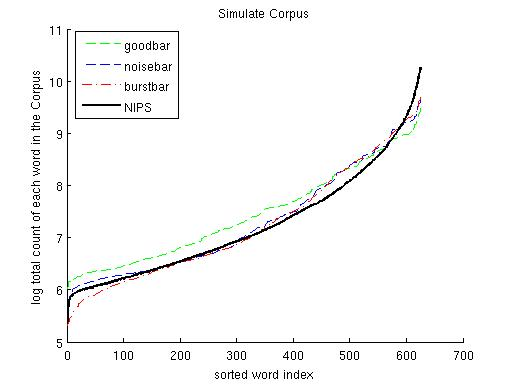
\includegraphics[width=3in,height=2.5in]{sc.jpg}\ 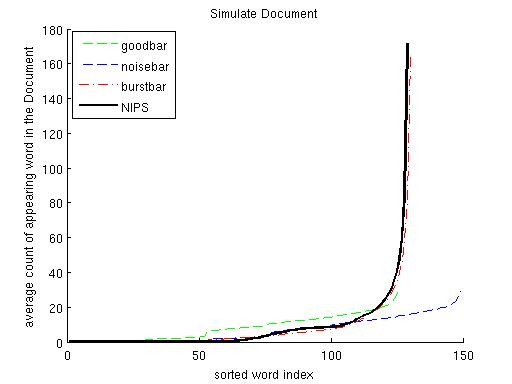
\includegraphics[width=3in,height=2.5in]{sd.jpg}\\
\end{center}
\subsection{2.2) Noisiness}
\begin{enumerate}
 \item Naive fix:\\
Compare results from Gibbs with same settings on the NIPS training data and its denoised version.
 \item HDP-UDM:\\
Compare results from ME with same settings under HDP-UDM and HDP-DM.
\end{enumerate}
\subsection{2.3) Burstiness}
\begin{enumerate}
 \item No naive fix but we can show it is problematic for HDP-DM by encouraging small biased tables to be new topics. 
 \item Leave it for later development
\end{enumerate}


\end{spacing}
\end{document}

%%%%%%%%%%%%%%%%%%%%%%%%%%%%%%%%%%%%%%%%%%%%%%%%%%%%%%%%%%%%%
